\subsection{Höhere Momente}
\hypertarget{Sec:MomGenFun}{}

Wir können die Definition des Erwartungswertes nun verallgemeinern.

\begin{Definition}{($n$-tes Moment)}
Sei $(\Omega, \mathscr{A}, \mathbb{P})$ ein Wahrscheinlichkeitsraum und $X$ eine reelle Zufallsvariable. Zu $n \in \mathbb{N}$ definiert man das \textit{$n$-te Moment von $X$} \en{moment} durch
\[\mathbb{E}(X^n) := \int X^n \d \mathbb{P}~.\]
\end{Definition}

Auf die Bemerkung zur Berechnung wollen wir an dieser Stelle verzichten. Wir werden dies sofort programmieren.

\begin{Code}{(\lstinline|_moment_integration|)}
\hypertarget{Code:n_Moment_Integration}{}Wollen wir die Berechnung des $n$-ten Moments in Python implementieren, so müssen wir zuerst das \hyperlink{Dichtekorollar}{\blue{Dichtekorollar}} anwenden und erhalten ein analoges Ergebnis zum \hyperlink{Bem:Berechnung_Erwartung}{\blue{Erwartungswert}}. Wir müssen nur $X$ durch $X^n$ beziehungsweise $x$ durch $x^n$ ersetzen. Da wir für die verschiedenen Typen jeweils eine \hyperlink{Code:Integrate}{\blue{Integrationsmethode}} definiert haben, ist die Berechnung des $n$-ten Moments sehr einfach.
\begin{lstlisting}
def _moment_integration(self, n):
    moment = self.integrate_random_variable(self.variable**n)
    return moment
\end{lstlisting}
Diese Methode geht zurück in die jeweilige Unterklasse und integriert beziehungsweise summiert dann die $n$-te Potenz der Variable und multipliziert dies anschließend mit der Dichte. Wie definiert, wird dies dann entsprechend vereinfacht und aufgeräumt. An dieser Stelle sieht man wunderschön die Eleganz, die wir durch die klasseninterne \lstinline|integrate_random_variable|-Methode gewonnen haben.
\end{Code}

Diese Methode können wir gleich ausprobieren.

\begin{Beispiel}{($n$-tes Moment Regen)}
Wir wollen nun für das \hyperlink{Bsp:Regen}{\blue{Regenbeispiel}} das $n$-te Moment berechnen. Betrachte
\begin{align*}
\mathbb{E}(X^n) &= \int_\mathbb{R} x^n \indi_{[0, 1]}(x) \d x\\
&= \int_0^1 x^n \d x\\
&= \left[ \frac{x^{n+1}}{n + 1} \right]_0^1\\
&= \frac{1}{n + 1} - 0\\
&= \frac{1}{n + 1}~.
\end{align*}
Für $n = 1$ erhalten wir den \hyperlink{Bsp:ErwRegen}{\blue{zuvor}} berechneten Erwartungswert von $1/2$. Wir können nun unserem Ergebnis überprüfen
\begin{lstlisting}[numbers=left, numberstyle=\tiny\color{codegray}]
x = sym.Symbol('x', real=True)
n = sym.Symbol('n', integer=True, positive=True)
density = sym.Integer(1)
rv = RandomVariableContinuous(density, x, supp=[sym.Integer(0), sym.Integer(1)])
moment = rv.moment(n)
\end{lstlisting}
und wir erhalten tatsächlich \lstinline|1/(n + 1)|.
\end{Beispiel}

\newpage

Wir haben nun schon an einigen Stellen als Voraussetzung den Begriff der Integrierbarkeit benötigt. Dies wollen wir an dieser Stelle definieren.

\begin{Definition}{(Integrierbarkeit und $n$-tes absolutes Moment)}
Sei $(\Omega, \mathscr{A}, \mathbb{P})$ ein Wahrscheinlichkeitsraum und $X$ eine reelle Zufallsvariable. Man nennt $X$ \textit{$n$-mal integrierbar}, falls gilt
\[\dabs{X}_n := \mathbb{E}(\abs{X}^n)^\frac{1}{n} < \infty~.\]
Man bezeichnet $\mathbb{E}(\abs{X}^n)$ auch als \textit{$n$-tes absolutes Moment} \en{absolute moment}.
\end{Definition}

Wir werden die Implementierung dieser Methode nicht vorführen, da im Vergleich zur vorigen Methode nur \lstinline|self.variable**n| durch \lstinline|sym.Abs(self.variable)**n| ersetzt wird. Auf ein Beispiel wollen wir jedoch nicht verzichten.

\begin{Beispiel}{($n$-tes absolutes Moment Exponentialverteilung)}
Sei $X \sim \Exp(\lambda)$ mit $\lambda > 0$ exponentialverteilt. Wir berechnen das erste absolute Moment von Hand. Betrachte
\begin{align*}
\mathbb{E}(\abs{X}) &= \int_\mathbb{R} \abs{x} \lambda \exp(- \lambda x) \indi_{[0, \infty)} \d x\\
&= \int_0^\infty \lambda \abs{x} \exp(- \lambda x) \d x~.
\intertext{Da wir $x$ nur auf $[0, \infty)$ betrachten und dies dort nichtnegativ ist, können wir den Betrag weglassen und erhalten}
&= \int_0^\infty \lambda x \exp(- \lambda x) \d x~.
\intertext{Mit partieller Integration erhalten wir}
&= \left[ - x \exp(- \lambda x) \right]_0^\infty + \int_0^\infty 1 \exp(- \lambda x) \d x\\
&= \left[ - 0 + 0 \right] + \int_0^\infty \exp(- \lambda x) \d x\\
&= \left[ - \frac{1}{\lambda} \exp(- \lambda x) \right]_0^\infty\\
&= - 0 + \frac{1}{\lambda}\\
&= \frac{1}{\lambda}~.
\end{align*}
Verwenden wir nun
\begin{lstlisting}[numbers=left, numberstyle=\tiny\color{codegray}]
lamda = sym.symbols('lambda', real=True, positive=True)
x = sym.symbols('x', real=True)
density = lamda * sym.exp(- lamda * x)
rv = RandomVariableContinuous(density, x, supp=[sym.Integer(0), sym.oo])
absolute_moment = rv.absolute_moment(1)
\end{lstlisting}
so erhalten wir ebenso \lstinline|1/lambda|. Wollten wir nun aber allgemein für $n \in \mathbb{N}$ das $n$-te absolute Moment berechnen, so würden wir nach einer kurzen Rechnung von Hand feststellen, dass wir $n$-mal partiell integrieren müssen. Viel einfacher ist es an den folgenden Teil anzufügen
\begin{lstlisting}[numbers=left, numberstyle=\tiny\color{codegray}, firstnumber=6]
n = sym.symbols('n', integer=True, nonnegative=True)
general_absolute_moment = rv.absolute_moment(n)
\end{lstlisting}
Wir erhalten \lstinline|factorial(n)/lambda**n|. Also ist
\[\mathbb{E}(\abs{X}^n) = \frac{n!}{\lambda^n}\]
Somit existieren zur Exponentialverteilung absolute Momente beliebiger Ordnung. Insbesondere stimmen die absoluten und die rohen Momente überein.
\end{Beispiel}

\vspace*{-\medskipamount}

\begin{Satz}{(Integrierbarkeit)}
\hypertarget{Satz:Integrierbarkeit}{}Sei $(\Omega, \mathscr{A}, \mathbb{P})$ ein Wahrscheinlichkeitsraum und $X$ eine reelle Zufallsvariable. Ist $X$ $n$-mal integrierbar, so ist $X$ auch $m$-mal integrierbar mit $m \leq n$.
\end{Satz}

\begin{Beweis}{}
Dies folgt aus der allgemeinen Schachtelung der $L^p$- beziehungsweise $\mathcal{L}^p$-Räume.
\end{Beweis}

\begin{Beispiel}{(Nicht-integrierbare Familie)}
\hypertarget{Bsp:Nicht-Int}{}Wir werden uns in diesem Beispiel mit einer Familie von Zufallsvariablen beschäftigen, die nur bis zu einem bestimmten Grad integrierbar sind. Sei zu $k \in \mathbb{N}_{> 1}$ die Dichte von $X_k$ gegeben durch
\[\varphi_k(x) = c_k \frac{1}{1 + x^k} \indi_{[0, \infty)}(x)\]
für alle $x \in \mathbb{R}$. Wir werden in einem ersten Schritt die Konstanten $c_k$ bestimmen, damit diese Funktionen Dichten sind. Betrachte also
\begin{align*}
\mathbb{P}_{X_k}(\mathbb{R}) &= \int_\mathbb{R} c_k \frac{1}{1 + x^k} \indi_{[0, \infty)}(x) \d x\\
&= c_k \int_0^\infty \frac{1}{1 + x^k} \d x~.
\end{align*}
Dieses Integral ist leider nur für $k = 1, 2$ einfach lösbar. Wir verwenden also die Bibliothek.
\begin{lstlisting}[numbers=left, numberstyle=\tiny\color{codegray}]
x = sym.Symbol('x', real=True)
k = sym.Symbol('k', integer=True, positive=True)
density = 1 / (1 + x**k)
rv = RandomVariableContinuous(density, x, supp=[sym.Integer(0), sym.oo], force_density=True)
value = rv._is_density()
\end{lstlisting}
Wir erhalten
\begin{align*}
\mathbb{P}_{X_k}(\mathbb{R}) &= c_k \cdot \frac{\pi}{k \sin\left( \frac{\pi}{k} \right)}~.
\intertext{Da dies eins sein muss, erhalten wir äquivalent}
c_k &= \frac{k}{\pi} \sin\left( \frac{\pi}{k} \right)~.
\end{align*}
Also ist
\[\varphi_k(x) = \frac{k}{\pi} \sin\left( \frac{\pi}{k} \right) \frac{1}{1 + x^k} \indi_{[0, \infty)}(x)\]
eine Wahrscheinlichkeitsdichte. Diese ist nicht-negativ, da alle Faktoren nicht-negativ sind. Insbesondere ist auch der Sinus-Term nicht-negativ, da $\pi / k \in [0, \pi]$ ist für alle $k \in \mathbb{N}_{>1}$ und der Sinus dort nicht-negativ ist. Verwenden wir also
\begin{lstlisting}[numbers=left, numberstyle=\tiny\color{codegray}, firstnumber=6]
density = k / sym.pi * sym.sin(sym.pi / k) * 1 / (1 + x**k)
rv = RandomVariableContinuous(density, x, supp=[sym.Integer(0), sym.oo])
value = rv._is_density()
\end{lstlisting}
so erhalten wir \lstinline|1| und können auf \lstinline|force_density| verzichten. Die Warnung wegen dem Auflösen stückweisen Funktion erscheint, da $k > 1$ sein muss und wir dies mit SymPy leider nicht definieren können. Die Zufallsvariable $X_k$ ist nur $(k - 2)$-mal integrierbar. Betrachte für $n > k - 2$ mit dem \hyperlink{Kor:Dichtekorollar}{\blue{Dichtekorollar}}
\begin{align*}
\mathbb{E}\left( \abs{X_k}^n \right) &= \int_\mathbb{R} \abs{x^n} \frac{k}{\pi} \sin\left( \frac{\pi}{k} \right) \frac{1}{1 + x^k} \indi_{[0, \infty)}(x) \d x\\
&= \frac{k}{\pi} \sin\left( \frac{\pi}{k} \right) \int_0^\infty \frac{\abs{x^n}}{1 + x^k} \d x~.
\intertext{Da wir nur über die positive reelle Halbachse integrieren, können wir im Zähler den Betrag weglassen und wir erhalten}
&= \frac{k}{\pi} \sin\left( \frac{\pi}{k} \right) \int_0^\infty \frac{x^n}{1 + x^k} \d x~.
\intertext{Dies können wir Abschätzen}
&\geq \frac{k}{\pi} \sin\left( \frac{\pi}{k} \right) \int_0^\infty \frac{x^n}{x^k} \d x\\
&= \frac{k}{\pi} \sin\left( \frac{\pi}{k} \right) \int_0^\infty x^{n - k} \d x~.
\intertext{Integration liefert}
&= \frac{k}{\pi} \sin\left( \frac{\pi}{k} \right) \left[ \begin{cases}
\log(x), &n = k - 1\\
\frac{1}{n - k + 1} x^{n - k + 1}, & n > k - 1
\end{cases} \right]_0^\infty~.
\end{align*}
Beide Fälle divergieren. Somit ist diese Zufallsvariable für $n > k - 2$ nicht $n$-integrierbar. Verwenden wir SymPy zur Bestimmung des $(k - 2)$-ten absoluten Moments, so erhalten wir mit
\begin{lstlisting}[numbers=left, numberstyle=\tiny\color{codegray}, firstnumber=9]
moment = rv.absolute_moment(k - 2)
\end{lstlisting}
den Wert \lstinline|1|, weshalb die Zufallsvariable $(k - 2)$-mal integrierbar ist. Für die Abschätzung betrachten wir
\begin{align*}
\frac{x^n}{1 + x^k} &\geq \frac{x^n}{x^k}~.
\intertext{Erweitern wir zum gemeinsamen Nenner, so erhalten wir}
\frac{x^n x^k}{(1 + x^k) x^k} &\geq \frac{x^n (1 + x^k)}{x^k (1 + x^k)}~.
\intertext{Das Ungleichungszeichen bleibt erhalten, da sowohl $1 + x^k$ als auch $x^k$ auf $[0, \infty)$ nicht-negativ sind. Bringen wir beides auf dieselbe Seite, so gilt}
0 &\geq \frac{x^n (1 + x^k) - x^n x^k}{x^k (1 + x^k)}\\
&\geq \frac{x^n + x^n x^k - x^n x^k}{x^k (1 + x^k)}\\
&\geq \frac{x^n}{x^k (1 + x^k)}~,
\end{align*}
da alle Faktoren nicht-negativ sind. An dieser Stelle sei nochmals eine Warnung bezüglich dem Auflösen von stückweisen Funktionen gegeben. Verwenden wir direkt
\begin{lstlisting}[numbers=left, numberstyle=\tiny\color{codegray}, firstnumber=10]
n = sym.Symbol('n', integer=True, positive=True)
moment = rv.absolute_moment(n)
\end{lstlisting}
so erhalten wir neben der Warnung \lstinline|-sin(pi/k)/sin(pi*(k + n + 1)/k)|. Setzen wir hier $n = k$, so erhielten wir fälschlicherweise \lstinline|-1|.

\newpage

Verwenden wir
\begin{lstlisting}[numbers=left, numberstyle=\tiny\color{codegray}, firstnumber=12]
RandomVariable.no_chopping()
moment = rv.absolute_moment(n)
\end{lstlisting}
so erhalten wir die folgende, richtige Funktion für die absoluten Momente
\[\mathbb{E}\left( \abs{X_k}^n \right) = \begin{cases}
- \frac{\sin\left( \frac{\pi}{k} \right)}{\sin\left( \frac{\pi (k + n + 1)}{k} \right)}, &\frac{n + 1}{k} < 1\\
\frac{k \sin\left(\frac{\pi}{k} \right) \int_0^\infty \frac{\abs{x}^n}{x^k + 1} \d x}{\pi}, &\text{sonst}~.
\end{cases}\]
Die Bedingung ist $n < k - 1$, wie von uns gefordert. Nach dem \hyperlink{Satz:Integrierbarkeit}{\blue{Satz zur Integrierbarkeit}} hätte es mittels Negation schon genügt zu zeigen, dass $\mathbb{E}(\abs{X_k}^{k - 1})$ nicht endlich ist. Somit sind auch alle höheren absoluten Momente nicht mehr endlich. Man sollte sich immer davon überzeugen, ob das Ergebnis von SymPy Sinn ergibt, falls man diese Warnung bekommt. Dennoch ist es sehr sinnvoll, stückweise Funktionen zu kürzen, da dies in den meisten Fällen natürliche Beschränkungen wie $p \in (0, 1)$ oder ähnliches sind.
\end{Beispiel}

Man könnte vermuten, dass es einen Satz gibt, der besagt, dass zu einer $n$-fach integrierbaren Zufallsvariable auch das $n$-te Moment existiert. Hierzu betrachten wir das folgende Gegenbeispiel.

\begin{Beispiel}{(Cauchy-Verteilung)}
Sei $X$ Cauchy-verteilt. Seien dazu $x_0 \in \mathbb{R}$ und $\gamma > 0$. Die Dichte ist dann für $x \in \mathbb{R}$ gegeben durch
\[\varphi(x) = \frac{1}{\pi \gamma} \left( 1 + \frac{(x - x_0)^2}{\gamma^2} \right)^{-1}~.\]
Im einfachsten Fall von $\gamma = 1$ und $x_0 = 0$ finden wir
\begin{align*}
\varphi(x) &= \frac{1}{\pi} \left( 1 + x^2 \right)^{-1}\\
&= \frac{1}{\pi} \frac{1}{1 + x^2}~.
\end{align*}
Dies ist fast ein Vertreter der \hyperlink{Bsp:Nicht-Int}{\blue{obigen}} nicht-integrierbaren Familie. Die Cauchy-Verteilung ist aber auf ganz $\mathbb{R}$ und nicht nur auf $[0, \infty)$ definiert. Es lässt sich zeigen, dass $\dabs{X}_1 < \infty$ ist und $X$ somit integrierbar ist. Betrachten wir hingeben $\mathbb{E}(X)$, so ist dies nicht definiert. Auch SymPy hat mit diesem Integral Probleme. Verwenden wir
\begin{lstlisting}[numbers=left, numberstyle=\tiny\color{codegray}]
x = sym.Symbol('x', real=True)
x_0 = sym.Integer(0)
gamma = sym.Integer(1)
density = 1 / (sym.pi * gamma) * 1 / (1 + (x - x_0)**2 / gamma**2)
rv = RandomVariableContinuous(density, x)
absolute_moment = rv.absolute_moment(1) 
\end{lstlisting}
so lässt SymPy den Ausdruck für das erste absolute Moment stehen ohne ihn weiter auszuwerten. Verwenden wir nun
\begin{lstlisting}[numbers=left, numberstyle=\tiny\color{codegray}, firstnumber=7]
absolute_moment = sym.N(absolute_moment)
\end{lstlisting}
zur numerischen Berechnung, so erhalten wir \lstinline|100|. Dieser Wert ist auf jeden Fall endlich. Lassen wir nun mit
\begin{lstlisting}[numbers=left, numberstyle=\tiny\color{codegray}, firstnumber=8]
mean = rv.mean()
\end{lstlisting}
den Erwartungswert berechnen, so erhalten wir \lstinline|nan|. Für eine Cauchy-verteilte Zufallsvariable scheinen also die absoluten Momente endlich zu sein, ohne dass die entsprechenden rohen Moment existieren.
\end{Beispiel}

Auf die Frage der Integrierbarkeit wollen wir im Folgenden verzichten. Wir versuchen mit dem Programm entsprechende Moment zu berechnen und falls diese endlich sind, gibt SymPy uns hoffentlich das entsprechende Ergebnis. Ansonsten erhalten wir andere SymPy-Objekte, die wir nun kurz besprechen werden.

\begin{Bemerkung}{(Unbestimmte Werte) \cite{SymPy}}
SymPy unterscheidet die unbestimmte Werte auf die folgenden Arten.
\begin{enumerate}[label=(\roman*)]
\item \lstinline|nan|: Für nicht-definierte Ausdrücke, denen man keinen Wert \en{indeterminate form} zuordnen kann, wie $0/0$ oder $\infty - \infty$, gibt SymPy ein \lstinline|nan|-Objekt zurück. Dies steht für keine Zahl \en{not a number}. Es sei erwähnt, dass die klassischerweise nicht-definierten Ausdrücke $0^0$ und $\infty^0$ wie in Python üblich zu Eins ausgewertet werden.

\item \lstinline|oo|: Für nicht-endliche Werte gibt SymPy \lstinline|oo| für $\infty$ oder \lstinline|-oo| für $- \infty$ zurück. Dies ist beispielsweise der Fall für $\int_0^\infty x \d x$ respektive $\int_{-\infty}^0 x \d x$.

\item \lstinline|zoo|: Für nicht-endliche Werte im komplexen gibt SymPy \lstinline|zoo| zurück. Dies ist eine komplexe Zahl von unendlichem Betrag mit unbekannter Phase. Dies tritt beispielsweise bei $1 / 0$ auf. Wir erhalten ein solches Objekt, falls SymPy auf dem Weg der Berechnung irgendwann versucht etwas im Komplexen zu berechnen oder zu vereinfachen. Dies tritt also häufig im Zusammenhang mit der Exponentialfunktion auf.
\end{enumerate}
\end{Bemerkung}

Wir können nun eine weitere Art von Momenten definieren.

\begin{Definition}{(Zentralmoment)}
Sei $(\Omega, \mathscr{A}, \mathbb{P})$ ein Wahrscheinlichkeitsraum und $X$ eine $n$-mal integrierbare Zufallsvariable. Zu $n \in \mathbb{N}$ definiert man das \textit{$n$-te Zentralmoment von $X$} \en{central moment} durch
\[\mu_n := \mathbb{E}\left((X - \mathbb{E}(X))^n\right)~.\]
\end{Definition}

\begin{Code}{(\lstinline|_central_moment_integration|)}
Auch hier ist die Implementierung dank Vorarbeit sehr einfach.
\begin{lstlisting}
def _central_moment_integration(self, n):
    mean = self.mean()
    central_moment = self.integrate_random_variable((self.variable - mean)**n)
    return central_moment
\end{lstlisting}
Betrachten wir nun beispielsweise eine stetige Zufallsvariable mit Dichte $\varphi$. Dann gilt
\begin{align*}
\mu_n &= \mathbb{E}\left((X - \mathbb{E}(X))^n\right)\\
&= \int (X - \mathbb{E}(X))^n \d \mathbb{P}~.
\intertext{Verwenden wir nun das \hyperlink{Kor:Dichtekorollar}{\blue{Dichtekorollar}}, so erhalten wir mit $\mu = \mathbb{E}(X)$}
&= \int_\mathbb{R} (x - \mu)^n \varphi(x) \d x~.
\end{align*}
Die Integrationsmethode berechnet dasselbe. Die \lstinline|mean|-Methode bestimmt den Erwartungswert. Dieser wird entweder mittels \hyperlink{Code:n_Moment_Integration}{\blue{\lstinline|_moment_integration|}} oder mit einer \hyperlink{Code:n_Moment_Generating}{\blue{anderen Methode}} berechnet, welche wir noch \hyperlink{Kor:Momente_MomGenFun}{\blue{später}} entwickeln werden.
\end{Code}

\newpage

\begin{Beispiel}{(Zentralmomente)}
\begin{enumerate}[label=(\roman*)]
\item \hypertarget{Bsp:Zentra}{}Sei $X \sim \Ber(p)$ mit $p \in (0, 1)$ Bernoulli-verteilt. Wir werden nun das sechste Zentralmomente berechnen. Betrachte mit $E = \{0, 1\}$
\begin{align*}
\mu_6 &= \sum_{n \in E} \left(n - \mathbb{E}(X)\right)^6 \mathbb{P}(X = n)~.
\intertext{Wir kennen bereites $\mathbb{E}(X) = p$, es folgt also}
&= \sum_{n \in E} \left(n - p\right)^6 \mathbb{P}(X = n)\\
&= \left(0 - p\right)^6 \mathbb{P}(X = 0) + (1 - p)^6 \mathbb{P}(X = 1)\\
&= p^6 (1 - p) + (1 - p)^6 p\\
&= p^5 p (1 - p) + (1 - p)^6 p (1 - p)\\
&= p^6 - p^7 + (p^6 - 6 p^5 + 15 p^4 - 20 p^3 + 15 p^2 - 6 p + 1) p\\
&= p^6 - p^7 + p^7 - 6 p^6 + 15 p^5 - 20 p^4 + 15 p^3 - 6 p^2 + p\\
&= - 5 p^6 + 15 p^5 - 20 p^4 + 15 p^3 - 6 p^2 + p~.
\end{align*}
Verwenden wir
\begin{lstlisting}[numbers=left, numberstyle=\tiny\color{codegray}]
p = sym.Symbol('p', real=True, positive=True)
n = sym.Symbol('n', integer=True, nonnegative=True)
density = {1: p, 0: 1 - p}
rv = RandomVariableFinite(density, n)
sixth_central_moment = rv.central_moment(6)
sixth_central_moment = sym.expand(sixth_central_moment)
\end{lstlisting}
so erhalten wir ebenfalls \lstinline|-5*p**6 + 15*p**5 - 20*p**4 + 15*p**3 - 6*p**2 + p|.

\item Sei nun $X \sim \Poiss(\lambda)$ mit $\lambda > 0$ Poisson-verteilt. Die Zähldichte ist für $n \in \mathbb{N}_0$ gegeben durch
\[\varphi(n) = \frac{\lambda^n}{n!} \exp(- \lambda)~.\]
Wir bestimmen das zweite Zentralmoment. Betrachte also nach \cite{Joram}
\begin{align*}
\mathbb{E}\left( X (X - 1) \right) &= \sum_{n = 0}^\infty n (n - 1) \mathbb{P}(X = n)\\
&= \sum_{n = 0}^\infty n (n - 1) \frac{\lambda^n}{n!} \exp(- \lambda)~.
\intertext{Wir können die Terme für $n = 0$ und $n = 1$ weglassen, da diese null sind. Damit folgt}
&= \exp(- \lambda) \sum_{n = 2}^\infty n (n - 1) \frac{\lambda^n}{n \cdot (n-1) \cdot (n - 2)!}\\
&= \exp(- \lambda) \sum_{n = 2}^\infty \frac{\lambda^2 \lambda^{n - 2}}{(n - 2)!}\\
&= \lambda^2 \exp(- \lambda) \sum_{n = 2}^\infty \frac{\lambda^{n - 2}}{(n - 2)!}~.
\intertext{Ein Indexshift führt nun zu}
&= \lambda^2 \exp(- \lambda) \sum_{n = 0}^\infty \frac{\lambda^{n}}{(n)!}~.
\intertext{Die hinter Summe ist genau die Definition der Exponentialfunktion, womit folgt}
&= \lambda^2 \exp(- \lambda) \exp(\lambda)\\
&= \lambda^2~.
\end{align*}
Betrachte nun
\begin{align*}
\mathbb{E}\left( X (X - 1) \right) &= \mathbb{E}(X^2 - X)\\
&= \mathbb{E}(X^2) - \mathbb{E}(X)~.
\intertext{Mit $\mathbb{E}(X) = \lambda$ folgt dann}
&= \mathbb{E}(X^2) - \lambda
\intertext{und äquivalent}
\mathbb{E}(X^2) &= \mathbb{E}\left( X (X - 1) \right) + \lambda~.
\intertext{Einsetzen der obigen Rechnung liefert}
&= \lambda^2 + \lambda~.
\end{align*}
Wir finden damit
\begin{align*}
\mu_2 &= \mathbb{E}(X^2) - \mathbb{E}(X)^2\\
&= \lambda^2 + \lambda - \lambda^2\\
&= \lambda~.
\end{align*}
Mit
\begin{lstlisting}[numbers=left, numberstyle=\tiny\color{codegray}]
lamda = sym.Symbol('lambda', real=True, positive=True)
n = sym.Symbol('n', integer=True, nonnegative=True)
density = lamda**n / sym.factorial(n) * sym.exp(- lamda)
rv = RandomVariableDiscrete(density, n)
second_central_moment = rv.central_moment(2)
\end{lstlisting}
erhalten wir ebenfalls \lstinline|lambda|.

\item Sei $X \sim \Exp(\lambda)$ mit $\lambda > 0$ exponentialverteilt. Wir berechnen nun das dritte Zentralmoment. Betrachte
\begin{align*}
\mu_3 &= \mathbb{E}\left( (X - \mathbb{E}(X))^3 \right)~.
\intertext{Verwenden wir $\mathbb{E}(X) = 1 / \lambda$ und das \hyperlink{Kor:Dichtekorollar}{\blue{Dichtekorollar}}, so erhalten wir}
&= \int_{- \infty}^\infty \left(x - \frac{1}{\lambda}\right)^3 \lambda \exp(- \lambda x) \indi_{[0, \infty)}(x) \d x\\
&= \int_0^\infty \lambda \left(x - \frac{1}{\lambda}\right)^3 \exp(- \lambda x) \d x~.
\displaybreak
\intertext{Partielle Integration liefert}
&= \left[ - \left(x - \frac{1}{\lambda}\right)^3 \exp(- \lambda x) \right]_0^\infty + \int_0^\infty 3 \left(x - \frac{1}{\lambda}\right)^2 \exp(- \lambda x) \d x\\
&= \left[ - 0 + \frac{1}{\lambda^3} \right] + \int_0^\infty 3 \left(x - \frac{1}{\lambda}\right)^2 \exp(- \lambda x) \d x\\
&= \frac{1}{\lambda^3} + \int_0^\infty 3 \left(x - \frac{1}{\lambda}\right)^2 \exp(- \lambda x) \d x~.
\intertext{Nochmal partielle Integration liefert}
&= \frac{1}{\lambda^3} + \left[ - \frac{3}{\lambda} \left(x - \frac{1}{\lambda}  \right)^2 \exp(- \lambda x) \right]_0^\infty + \int_0^\infty \frac{6}{\lambda} \left(x - \frac{1}{\lambda}\right) \exp(- \lambda x) \d x\\
&= \frac{1}{\lambda^3} + \left[ - 0 + \frac{3}{\lambda} \frac{1}{\lambda^2} \right] + \int_0^\infty \frac{6}{\lambda} \left(x - \frac{1}{\lambda}\right) \exp(- \lambda x) \d x\\
&= \frac{1}{\lambda^3} + \frac{3}{\lambda^3} + \int_0^\infty \frac{6}{\lambda} \left(x - \frac{1}{\lambda}\right) \exp(- \lambda x) \d x\\
&= \frac{2}{\lambda^3} + \int_0^\infty \frac{6}{\lambda} \left(x - \frac{1}{\lambda}\right) \exp(- \lambda x) \d x~.
\intertext{Ein letztes Mal partielle Integration liefert}
&= \frac{2}{\lambda^3} + \left[ - \frac{6}{\lambda^2} \left(x - \frac{1}{\lambda}\right) \exp(- \lambda x) \right]_0^\infty + \int_0^\infty \frac{6}{\lambda^2} \exp(- \lambda x) \d x\\
&= \frac{2}{\lambda^3} + \left[ - 0 - \frac{6}{\lambda^2} \frac{1}{\lambda} \right] + \int_0^\infty \frac{6}{\lambda^2} \exp(- \lambda x) \d x\\
&= \frac{2}{\lambda^3} - \frac{6}{\lambda^3} + \int_0^\infty \frac{6}{\lambda^2} \exp(- \lambda x) \d x\\
&= - \frac{4}{\lambda^3} + \int_0^\infty \frac{6}{\lambda^2} \exp(- \lambda x) \d x~.
\intertext{Dies können wir nun endlich mit dem Hauptsatz integrieren}
&= - \frac{4}{\lambda^3} + \left[ - \frac{6}{\lambda^3} \exp(- \lambda x) \right]_0^\infty\\
&= - \frac{4}{\lambda^3} + \left[ - 0 + \frac{6}{\lambda^3} \right]\\
&= - \frac{4}{\lambda^3} + \frac{6}{\lambda^3}\\
&= \frac{2}{\lambda^3}
\end{align*}
Mittels
\begin{lstlisting}[numbers=left, numberstyle=\tiny\color{codegray}]
x = sym.Symbol('x', real=True)
lamda = sym.Symbol('lambda', real=True, positive=True)
density = lamda * sym.exp(- lamda * x)
rv = RandomVariableContinuous(density, x, [sym.Integer(0), sym.oo])
third_central_moment = rv.central_moment(3)
\end{lstlisting}
erhalten wir ebenfalls \lstinline|2/lambda**3|.
\end{enumerate}
\end{Beispiel}

\newpage

Wir werden nun sehen, dass einige Zentralmomente für beliebige Verteilungen gleich sind.

\begin{Bemerkung}{(Triviale Zentralmomente)}
\hypertarget{Bem:Zentralmomente}{}Das nullte Zentralmoment einer Zufallsvariable ist immer eins. Betrachte
\begin{align*}
\mu_0 &= \mathbb{E}\left((X - \mathbb{E}(X))^0\right)\\
&= \mathbb{E}(1)\\
&= \int \varphi(x) \d x
\intertext{Da $\varphi$ eine Dichtefunktion einer Zufallsvariable ist, gilt nach \hyperlink{Def:Maß}{\blue{Definition von Wahrscheinlichkeitsmaßen}}}
&= 1~.
\end{align*}
Diese Aussage können wir auch fast vollständig mit SymPy \glqq beweisen\grqq{}.
\begin{lstlisting}[numbers=left, numberstyle=\tiny\color{codegray}]
x = sym.Symbol('x', real=True)
density = sym.Function('varphi')(x)
rv = RandomVariableContinuous(density, x, force_density=True)
zeroth_central_moment = rv.central_moment(0)
\end{lstlisting}
Wir erhalten dann \lstinline|Integral(varphi(x), (x, -oo, oo))|, was das Integral über die Dichte ist. Da wir eine Wahrscheinlichkeitsdichte verwendet haben, ist dies wie gefordert eins. Diesen letzten Schritt haben wir leider selbst machen müssen, da wir SymPy nicht erklären können, dass die Dichtefunktion normiert ist.\\

Das erste Zentralmoment einer integrierbaren Zufallsvariable verschwindet immer. Betrachte
\begin{align*}
\mu_1 &= \mathbb{E}\left((X - \mathbb{E})^1\right)\\
&= \mathbb{E}\left(X - \mathbb{E}(X)\right)~.
\intertext{Da das Integral linear ist, folgt}
&= \mathbb{E}(X) - \mathbb{E}(X)\\
&= 0~.
\end{align*}
Dies können wir leider nicht mit SymPy \glqq beweisen\grqq{}, da es keine Möglichkeit gibt SymPy zu erklären, dass der Erwartungswert endlich ist. Somit möchte SymPy das Integral nicht auseinanderziehen und vereinfachen.
\end{Bemerkung}

Das erste nicht-triviale Zentralmoment ist also das zweite. Dieses bekommt sogar einen speziellen Namen.

\begin{Definition}{(Varianz und Standardabweichung)}
Sei $(\Omega, \mathscr{A}, \mathbb{P})$ ein Wahrscheinlichkeitsraum und $X$ eine reelle, zweimal integrierbare Zufallsvariable. Die Varianz \en{variance} ist definiert durch
\begin{align*}
\Var(X) &:= \mu_2\\
&= \mathbb{E}\left( (X - \mathbb{E}(X))^2 \right)~.
\end{align*}
Damit definiert man die Standardabweichung \en{standard deviation} durch
\[\sigma := \sqrt{\Var(X)}~.\]
Man kann also auch $\Var(X) = \sigma^2$ schreiben.
\end{Definition}

Auf die Implementierung dieser neuen Definitionen wollen wir an dieser Stelle verzichten, da wir die allgemeineren Funktionen bereits definiert haben.

\begin{Beispiel}{(Interpretation Standardabweichung) \cite{Joram}}
\hypertarget{Bsp:Normal_std}{}Wie bei \hyperlink{Bsp:InterpretErw}{\blue{der Interpretation des Erwartungswertes}} wollen wir an dieser Stelle ebenfalls versuchen dieses Zentralmoment zu interpretieren. Sei $X \sim \Nor(\mu, \sigma)$ mit $\mu \in \mathbb{R}$ und $\sigma > 0$ normalverteilt. Die Dichte ist gegeben durch
\[\varphi(x) = \frac{1}{\sqrt{2 \pi} \sigma} \exp\left( - \frac{1}{2} \frac{(x - \mu)^2}{\sigma^2} \right)~.\]
Um den riesigen Vorteil von SymPy zu zeigen, werden wir die Berechnung an dieser Stelle einmal von Hand durchführen. Betrachte nun
\begin{align*}
\Var(X) &= \mathbb{E}\left( (X - \mathbb{E}(X))^2 \right)\\
&= \int_{-\infty}^\infty (x - \mu)^2 \frac{1}{\sqrt{2 \pi} \sigma} \exp\left( - \frac{1}{2} \frac{(x - \mu)^2}{\sigma^2} \right) \d x\\
&= \frac{1}{\sqrt{2 \pi} \sigma} \int_{-\infty}^\infty (x - \mu)^2 \exp\left( - \frac{1}{2} \frac{(x - \mu)^2}{\sigma^2} \right) \d x~.
\intertext{Substituieren wir nun $z = x - \mu$, so ist $\d z = \d x$ und wir erhalten}
&= \frac{1}{\sqrt{2 \pi} \sigma} \int_{-\infty}^\infty z^2 \exp\left( - \frac{1}{2} \frac{z^2}{\sigma^2} \right) \d z~.
\intertext{Substituieren wir nun $z = \sqrt{2} \sigma x$, so ist $\d z = \sqrt{2} \sigma \d x$ und wir erhalten}
&= \frac{1}{\sqrt{2 \pi} \sigma} \int_{-\infty}^\infty (\sqrt{2} \sigma x)^2 \exp\left( - \frac{1}{2} \frac{(\sqrt{2} \sigma x)^2}{\sigma^2} \right) \sqrt{2} \sigma \d x\\
&= \frac{1}{\sqrt{2 \pi} \sigma} \int_{-\infty}^\infty 2 \sigma^2 x^2 \exp\left( - \frac{1}{2} \frac{2 \sigma^2 x^2}{\sigma^2} \right) \sqrt{2} \sigma \d x~.
\intertext{Durch Kürzen erhalten wir nun}
&= \frac{2 \sigma}{\sqrt{\pi}} \int_{-\infty}^\infty x^2 \exp\left( x^2 \right) \d x~.
\intertext{Der Integrand ist symmetrisch um Null. Wir können das Integral also umschreiben zu}
&= \frac{2 \sigma}{\sqrt{\pi}} 2 \int_0^\infty x^2 \exp\left( x^2 \right) \d x\\
&= \frac{4 \sigma}{\sqrt{\pi}} \int_0^\infty x^2 \exp\left( x^2 \right) \d x~.
\intertext{Substituieren wir nun $z = x^2$, so ist $\d x = 1 / (2 \sqrt{z}) \d z$ und wir erhalten}
&= \frac{4 \sigma}{\sqrt{\pi}} \int_0^\infty z \exp(z) \frac{1}{2 \sqrt{z}} \d z\\
&= \frac{2 \sigma}{\sqrt{\pi}} \int_0^\infty z^{\frac{3}{2} - 1} \exp(z) \d z~.
\displaybreak
\intertext{Verwenden wir nun die Definition der Gammafunktion mit $\Gamma(k) = \int_0^\infty z^{k - 1} \exp(- z) \d z$, so erhalten wir für $k = 3 / 2$}
&= \frac{2 \sigma}{\sqrt{\pi}} \Gamma\left( \frac{3}{2} \right)\\
&= \frac{2 \sigma}{\sqrt{\pi}} \frac{\sqrt{\pi}}{2}\\
&= \sigma~.
\end{align*}
Die Standardabweichung ist dann entsprechend $\sigma$. Verwenden wir nun SymPy, so benötigen wir
\begin{lstlisting}[numbers=left, numberstyle=\tiny\color{codegray}]
x = sym.Symbol('x', real=True)
mu = sym.Symbol('mu', real=True)
sigma = sym.Symbol('sigma', real=True, positive=True)
density = 1 / (sigma * sym.sqrt(2 * sym.pi)) * sym.exp(- (x - mu)**2 / (2 * sigma**2))
rv = RandomVariableContinuous(density, x)
variance = rv.variance()
std = rv.standard_deviation()
\end{lstlisting}
Wir erhalten ebenso \lstinline|sigma**2| und \lstinline|sigma|. Diese Berechnung hat je nach Computerleistung nur wenige Sekunden gedauert, während die händische Kalkulation deutlich mehr Zeit in Anspruch nimmt.\\

Anhand einer Normalverteilung kann man die Bedeutung der Varianz beziehungsweise der Standardabweichung leicht verstehen. Sie ist ein Maß für die Abweichung vom Erwartungswert. Wir werden nun im folgenden Bild sehen, wie die Größer der Standardabweichung den Plot der Dichtefunktion ändert.
\begin{figure}[H]
\centering
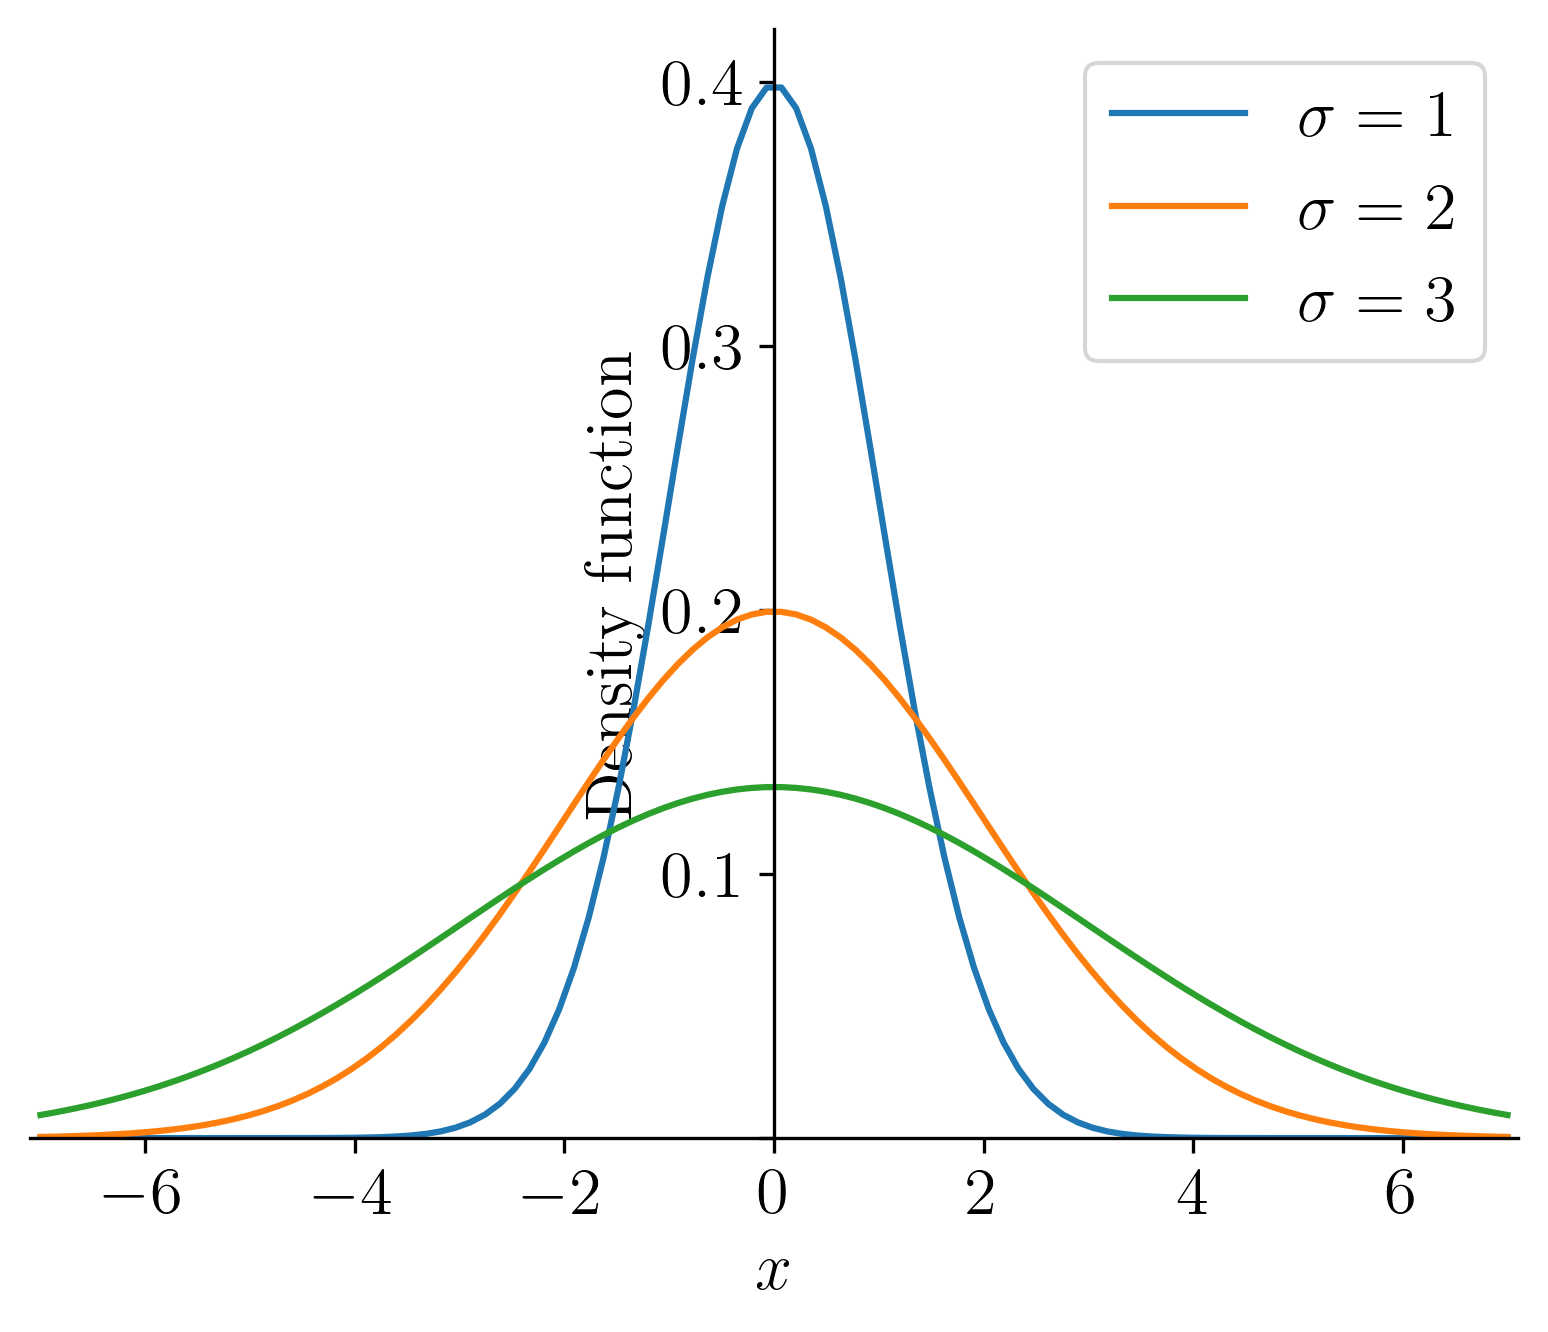
\includegraphics[width=0.5\linewidth]{./Section/Momente/Varianz Normalverteilung.png}
\caption{Dichte einer $\Nor(0, \sigma)$-Verteilung}
\end{figure}
Wie oben beschrieben führen große Standardabweichungen zu einer größeren Streuung um den Erwartungswert, welcher hier in der Null liegt.
\end{Beispiel}

\vspace*{-\medskipamount}

\begin{Bemerkung}{(Berechnung Varianz)}
In der obigen Definition ist die Varianz als ein Zentralmoment definiert. Wir können sie auch mittels der rohen Momente berechnen. Betrachte
\begin{align*}
\Var(X) &= \mathbb{E}\left( (X - \mathbb{E}(X))^2 \right)\\
&= \mathbb{E}\left( X^2 - 2 X \mathbb{E}(X) + \mathbb{E}(X)^2 \right)~.
\intertext{Mit der Linearität des Erwartungswertes folgt}
&= \mathbb{E}(X^2) - 2 \mathbb{E}(X) \mathbb{E}(X) + \mathbb{E}(X)^2\\
&= \mathbb{E}(X^2) - 2 \mathbb{E}(X)^2 + \mathbb{E}(X)^2\\
&= \mathbb{E}(X^2) - \mathbb{E}(X)^2~.
\end{align*}
Wir können die Varianz auch durch das zweite Moment minus das erste Moment zu Quadrat berechnen.
\end{Bemerkung}

Diese Aussage gilt sogar allgemeiner.

\begin{Satz}{(Darstellung der Zentralmomente)}
Sei $(\Omega, \mathscr{A}, \mathbb{P})$ ein Wahrscheinlichkeitsraum und $X$ eine reelle, $n$-mal integrierbare Zufallsvariable. Dann lässt sich das $n$-te Zentralmoment als Polynom der rohen Momente bis zum Grad $n$ darstellen. Es gilt
\[\mu_n = \sum_{k = 0}^n (-1)^k \begin{pmatrix}n \\ k\end{pmatrix} \mathbb{E}(X)^k \mathbb{E}(X^{n - k})~.\]
\end{Satz}

\begin{Beweis}{}
Betrachte
\begin{align*}
\mu_n &= \mathbb{E}\left( (X - \mathbb{E}(X))^n \right)~.
\intertext{Verwenden wir den binomische Lehrsatz, so erhalten wir}
&= \mathbb{E}\left( \sum_{k = 0}^n \begin{pmatrix}n \\ k\end{pmatrix} X^{n - k} (- \mathbb{E}(X))^k \right)\\
&= \mathbb{E}\left( \sum_{k = 0}^n (-1)^k \begin{pmatrix}n \\ k\end{pmatrix} X^{n - k} \mathbb{E}(X)^k \right)~.
\intertext{Da $X$ $n$-mal integrierbar ist flogt mit der Linearität des Erwartungswertes}
&= \sum_{k = 0}^n (-1)^k \begin{pmatrix}n \\ k\end{pmatrix} \mathbb{E}(X)^k \mathbb{E}(X^{n - k})~,
\end{align*}
was zu zeigen war.
\end{Beweis}

\begin{Bemerkung}{(Variationskoeffizient) \cite{Wiki:CV}}
Mit dem Begriff der Standardabweichung können wir den neuen Begriff des \textit{Variationskoeffizienten} \en{coefficient of variation} definieren. Es gilt, falls $\mathbb{E}(X) \neq 0$ ist
\[\VarK(X) := \frac{\sigma}{\mathbb{E}(X)}~.\]
In der Bibliothek ist er unter \lstinline|coefficient_of_variation| zu finden und wird unter Aufruf der Methoden \lstinline|mean| und \lstinline|standard_deviation| berechnet.
\end{Bemerkung}

\begin{Beispiel}{(Variationskoeffizient)}
Wir werden nun für ein Beispiel den Variationskoeffizient berechnen. Sei $X \sim \Nor(\mu, \sigma)$ normalverteilt mit $\mu \in \mathbb{R}$ und $\sigma > 0$. Den Erwartungswert werden wir an einer \hyperlink{Bsp:Normal_mean}{\blue{späteren Stelle}} noch berechnen. Die Standardabweichung kennen wir \hyperlink{Bsp:Normal_std}{\blue{bereits}}. Es gilt
\begin{align*}
\mathbb{E}(X) &= \mu\\
\Var(X) &= \sigma^2~.
\intertext{Damit können wir den Variationskoeffizienten berechnen}
\VarK(X) &= \frac{\sigma}{\mu}~.
\end{align*}

\newpage 

Um uns manuelle Berechnung zu ersparen, können wir auch
\begin{lstlisting}[numbers=left, numberstyle=\tiny\color{codegray}]
x = sym.symbols('x', real=True)
mu = sym.symbols('mu', real=True)
sigma = sym.symbols('sigma', real=True, positive=True)
density = 1 / (sigma * sym.sqrt(2 * sym.pi)) * sym.exp(- (x - mu)**2 / (2 * sigma**2))
rv = RandomVariableContinuous(density, x)
coefficient_of_variation = rv.coefficient_of_variation()
\end{lstlisting}
verwenden und erhalten ebenfalls \lstinline|sigma/mu|.
\end{Beispiel}

Mithilfe der Standardabweichung können wir nun die Zentralmomente entsprechend standardisieren.

\begin{Definition}{(Standardmoment)}
Sei $(\Omega, \mathscr{A}, \mathbb{P})$ ein Wahrscheinlichkeitsraum und $X$ eine $n$-mal integrierbare Zufallsvariable mit Standardabweichung $\sigma \neq 0$. Zu $n \in \mathbb{N}_{> 1}$ ist das \textit{$n$-te Standardmoment von $X$} \en{standardised moment} definiert durch
\begin{align*}
\tilde{\mu}_n &:= \frac{\mu_n}{\sigma^n}\\
&= \frac{\mathbb{E}\left( (X - \mathbb{E}(X))^n \right)}{\mathbb{E}\left( (X - \mathbb{E}(X))^2 \right)^n}~.
\end{align*}
\end{Definition}

\begin{Code}{(\lstinline|_standard_moment_integration|)}
Die Implementierung lehnt sich eher an die erste Schreibweise in der obigen Definition an.
\begin{lstlisting}
def _standard_moment_integration(self, n):
    central_moment = self.central_moment(n, use_integration=True)
    standard_deviation = self.standard_deviation(use_integration=True)
    standard_moment = central_moment / standard_deviation**n
    standard_moment = sym.simplify(standard_moment)
    return standard_moment
\end{lstlisting}
Wir bestimmen zuerst mit den entsprechenden Methoden das Zentralmoment und die Standardabweichung. Wie in der Definition dividieren wir diese und lassen dies nach Möglichkeit noch mit SymPy vereinfachen.
\end{Code}

\vspace*{-\medskipamount}

\begin{Bemerkung}{(Triviale Standardmomente)}
Ähnlich wie bei den Zentralmomenten ist das nullte Standardmoment immer eins. Betrachte
\begin{align*}
\tilde{\mu}_0 &= \frac{\mu_0}{\sigma^0}\\
&= \frac{1}{1}\\
&= 1.
\end{align*}
Für diese Tatsache können wir wieder einen \glqq Beweis\grqq{} mit SymPy führen.
\begin{lstlisting}[numbers=left, numberstyle=\tiny\color{codegray}]
x = sym.Symbol('x', real=True)
f = sym.Function('f')(x)
rv = RandomVariableContinuous(f, x, force_density=True)
zeroth_standardized_moment = rv.standard_moment(0)
\end{lstlisting}
Wir erhalten wie im \hyperlink{Bem:Zentralmomente}{\blue{Bemerkung zu den Zentralmomenten}} \lstinline|Integral(f(x), (x, -oo, oo))|, was aufgrund der Normiertheit einer Dichte genau eins ist.\\

Das erste Standardmoment ist null. Es gilt
\begin{align*}
\tilde{\mu}_1 &= \frac{\mu_1}{\sigma^1}\\
&= \frac{0}{\sigma}\\
&= 0~.
\end{align*}
Wie bei den \hyperlink{Bem:Zentralmomente}{\blue{Zentralmomenten}} können wir dies vermutlich aus ähnlichen Gründen nicht \glqq beweisen\grqq{}.

\newpage

Zu guter Letzt ist das zweite Standardmoment immer eins. Betrachte dazu
\begin{align*}
\tilde{\mu}_2 &= \frac{\mu_2}{\sigma^2}\\
&= \frac{\sigma^2}{\sigma^2}\\
&= 1
\end{align*}
Dies können wir wieder \glqq beweisen\grqq{} lassen. Durch das Anfügen von
\begin{lstlisting}[numbers=left, numberstyle=\tiny\color{codegray}, firstnumber=5]
second_standardized_moment = rv.standard_moment(2)
\end{lstlisting}
erhalten wir \lstinline|1|.
\end{Bemerkung}

\vspace*{-\medskipamount}

\begin{Bemerkung}{(Spezielle Standardmomente) \cite{Wiki:Mom}}
Analog zur Varianz gibt es auch hier Standardmomente, die einen speziellen Namen haben. Das dritte Standardmoment bezeichnet man als Schiefe \en{skewness} und das vierte als Wölbung \en{kurtosis}. Weniger gebräuchlich sind die Begriffe für das fünfte und sechste Standardmoment, nämlich \textit{Hyperschiefe} \en{hyperskewness} respektive Hypertailedness \en{hypertailedness}. Diese Methoden sind unter den entsprechenden englischen Begriffen implementiert. Auch hier möchte ich auf eine Vorstellung des Codes verzichten, da einfach die \lstinline|standard_moment|-Methode mit Parameter \lstinline|3| und \lstinline|4| beziehungsweise \lstinline|5| und \lstinline|6| aufgerufen wird.
\end{Bemerkung}

Wir werden nun anhand einiger Beispiele diese Standardmomente berechnen.

\begin{Beispiel}{(Standardmomente)}
\begin{enumerate}[label=(\roman*)]
\item Sei $X \sim \Ber(p)$ Bernoulli-verteilt mit $p \in (0, 1)$. Wir berechnen die Hypertailedness. Betrachte also
\begin{align*}
\tilde{\mu}_6 &= \frac{\mu_6}{\sigma^6}~.
\intertext{$\mu_6$ haben wir \hyperlink{Bsp:Zentra}{\blue{oben}} bereits berechnet und $\sigma^2 = p (1 - p)$. Damit folgt}
&= \frac{p^5 p (1 - p) + (1 - p)^6 p (1 - p)}{\sqrt{p (1 - p)}^6}\\
&= \frac{p^5 p (1 - p) + (1 - p)^6 p (1 - p)}{\left(p (1 - p)\right)^3}\\
&= \frac{p^5 + (1 - p)^6}{\left(p (1 - p)\right)^2}\\
&= \frac{p^6 - 5 p^5 + 15 p^4 - 20 p^3 + 15 p^2 - 6 p + 1}{p^4 - 2 p^3 + p^2}~.
\end{align*}
Durch
\begin{lstlisting}[numbers=left, numberstyle=\tiny\color{codegray}]
p = sym.Symbol('p', real=True, positive=True)
n = sym.Symbol('n', integer=True, nonnegative=True)
density = {1: p, 0: 1 - p}
rv = RandomVariableFinite(density, n)
hypertailedness = rv.hypertailedness()
\end{lstlisting}
erhalten wir auch \lstinline|(p**5 - (p - 1)**5)/(p**2*(p - 1)**2)|.

\newpage

\item Sei $X \sim \Exp(\lambda)$ mit $\lambda > 0$ exponentialverteilt. Wir berechnen die Schiefe. Betrachte also
\begin{align*}
\tilde{\mu}_3 &= \frac{\mu_3}{\sigma^3}~.
\intertext{Wir haben bereits $\mu_3 = 2 / \lambda^3$ berechnet. Mit $\sigma = 1 / \lambda$ folgt}
&= \frac{\frac{2}{\lambda^3}}{\frac{1}{\lambda^3}}\\
&= \frac{2 \lambda^3}{\lambda^3}\\
&= 2~.
\end{align*}
Mit
\begin{lstlisting}[numbers=left, numberstyle=\tiny\color{codegray}]
x = sym.Symbol('x', real=True)
lamda = sym.Symbol('lambda', real=True, positive=True)
density = lamda * sym.exp(- lamda * x)
rv = RandomVariableContinuous(density, x, [sym.Integer(0), sym.oo])
skewness = rv.skewness()
\end{lstlisting}
erhalten wir dasselbe Ergebnis. Es ist interessant, dass alle Exponentialverteilungen unabhängig von der Wahl von $\lambda$ gleich schief sind.

\item Sei $X \sim \Nor(\mu, \sigma)$ mit $\mu \in \mathbb{R}$ und $\sigma > 0$ normalverteilt. Wir werden an dieser Stelle Schiefe und Wölbung nicht von Hand berechnen. Mit
\begin{lstlisting}[numbers=left, numberstyle=\tiny\color{codegray}]
x = sym.Symbol('x', real=True)
lamda = sym.Symbol('lambda', real=True, positive=True)
density = lamda * sym.exp(- lamda * x)
rv = RandomVariableContinuous(density, x, [sym.Integer(0), sym.oo])
skewness = rv.skewness()
kurtosis = rv.kurtosis()
\end{lstlisting}
erhalten wir \lstinline|0| und \lstinline|3|.
\end{enumerate}
Weitere Beispiele lassen sich einfach mit dem Code selbst ausrechnen.
\end{Beispiel}

Wir wollen an dieser Stelle mögliche Interpretationen für die Schiefe und Wölbung finden.

\begin{Beispiel}{(Interpretation Schiefe und Wölbung)}
Die Schiefe ist ein Maß dafür, wie symmetrisch oder asymmetrisch eine Verteilung ist. Ist die Schiefe positive, so liegt mehr Masse rechts vom Erwartungswert. Umgekehrtes gilt für negative Schiefen. Wie wir in obigem Beispiel gesehen haben, verschwindet die Schiefe der Normalverteilung. Dies liegt daran, dass die Dichte symmetrisch um den Erwartungswert ist. Außerdem haben wir oben gesehen, dass die Schiefe einer Exponentialverteilung immer zwei ist. An der Dichtefunktion können wir schon erahnen, dass die Schiefe positive sein muss.\\

Die Wölbung ist ein Maß dafür, wie steil oder flach sich die Verteilung um den Erwartungswert verhält. Da die Wölbung einer Normalverteilung immer drei ist, kann man andere Verteilungen mit der Normalverteilung vergleichen, indem man den \textit{Exzess} \en{excess kurtosis} definiert. Diesen erhält man, indem man drei von der Wölbung der Zufallsvariable abzieht. Er dient als Vergleichswert, wie schnell die Enden einer Verteilung gegen Null abfallen und ist unter \lstinline|excess_kurtosis| zu finden. Verschwindet der Exzess, so bezeichnet man die Verteilung als \textit{mesokurtisch} \en{mesocurtic}. Dies ist zum Beispiel die Normalverteilung. Ist der Exzess positiv beziehungsweise negativ, so bezeichnet man die Verteilung als \textit{leptokurtisch} \en{leptokurtic} respektive \textit{platykurtisch} \en{platykurtic}. Eine Methode, die den Exzess einer parameterfreien Verteilung interpretiert, lässt sich unter \lstinline|interpret_excess_kurtosis| finden.

\begin{enumerate}[label=(\roman*)]
\item Betrachte eine $(\mu, \sigma)$-Normalverteilung. Verwenden wir
\begin{lstlisting}[numbers=left, numberstyle=\tiny\color{codegray}]
x = sym.Symbol('x', real=True)
mu = sym.Symbol('mu', real=True)
sigma = sym.Symbol('sigma', real=True, positive=True)
density = 1 / (sigma * sym.sqrt(2 * sym.pi)) * sym.exp(- (x - mu)**2 / (2 * sigma**2))
rv = RandomVariableContinuous(density, x)
rv.interpret_excess_kurtosis()
\end{lstlisting}
so erhalten wir \lstinline|The Distribution is mesokurtic|, wie erwartet.

\item Sei nun $X \sim \Exp(\lambda)$ mit $\lambda > 0$ exponentialverteilt. Wir würden erwarten, dass der Exzess negativ ist, da eine Exponentialfunktion nur in $\exp(-x)$ und die Normalverteilung mit $\exp(-x^2)$ schneller abfällt. Mit
\begin{lstlisting}[numbers=left, numberstyle=\tiny\color{codegray}]
lamda = sym.symbols('lambda', real=True, positive=True)
x = sym.Symbol('x', real=True)
density = lamda * sym.exp(- lamda * x)
rv = RandomVariableContinuous(density, x, [sym.Integer(0), sym.oo])
rv.interpret_excess_kurtosis()
\end{lstlisting}
erhalten wir \lstinline|The Distribution is leptokurtic|, wie vorhergesagt.

\item \hypertarget{Bsp:Platy}{} Um ein platykurtisches Beispiel zu finden, benötigen wir eine Dichte, die schneller als $\exp(- x^2)$ abfällt. Wir können beispielsweise $\exp(- x^4)$ verwenden. Wir beginnen mit
\begin{lstlisting}[numbers=left, numberstyle=\tiny\color{codegray}]
x = sym.Symbol('x', real=True)
density = sym.exp(- x**4)
rv = RandomVariableContinuous(density, x)
value = rv._is_density()
\end{lstlisting}
und erhalten \lstinline|gamma(1/4)/2| als Ergebnis der nicht-normierten Dichte. Eine Wahrscheinlichkeitsdichte ist also
\[\varphi(x) = \frac{2}{\Gamma\left( \frac{1}{4} \right)} \exp(- x^4)~.\]
Mit
\begin{lstlisting}[numbers=left, numberstyle=\tiny\color{codegray}, firstnumber=5]
density = sym.Integer(2) / sym.gamma(sym.Rational(1, 4)) * sym.exp(- x**4)
rv = RandomVariableContinuous(density, x)
rv.interpret_excess_kurtosis()
\end{lstlisting} erhalten wir \lstinline|The Distribution is platykurtic|. Dies ist genau so, wie wir die Verteilung \glqq gebaut\grqq{} haben.
\end{enumerate}
\end{Beispiel}

\vspace*{-\medskipamount}

Im nächsten Abschnitt werden wir die versprochene andere Möglichkeit finden, mit der man Momente berechnen kann.